% #############################################################################
% This is Chapter 4
% !TEX root = ../main.tex
% #############################################################################
% Change the Name of the Chapter i the following line
\fancychapter{Architecture}
\cleardoublepage
% The following line allows to ref this chapter
\label{chap:arch}

The objective of the system was to develop a device in a box format to enable users to establish safe channels of communication. This is achieved with a safe and secure device which is personal to each individual. In order to secure the communications between users, the device saves the user's sensitive data, such as keys, and performs all security critical operations.
The system is designed so that each user has it's own physical box.

% -----------------------------------------------------
% -----------------------------------------------------
\section{Components}\label{chap:arch:components}

The system architecture, depicted in figure~\ref{fig:components}, is composed of two main components: the physical box which responsible for securing the data, and the client software on the user's computer, which communicates with the box.

\begin{figure}[h]
    \centering
    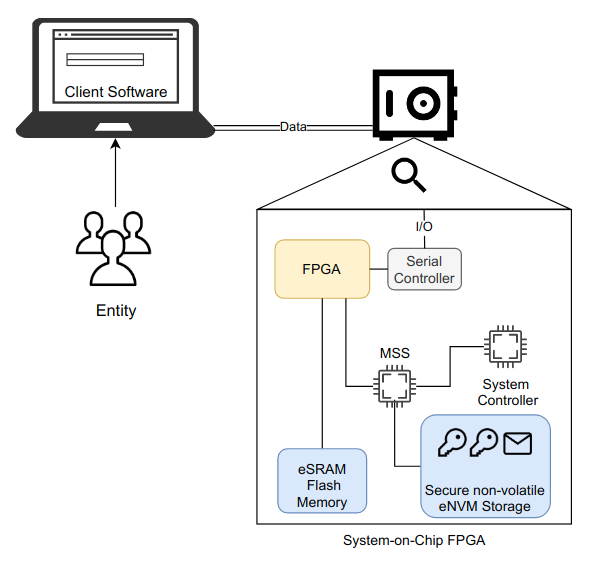
\includegraphics[width=0.7\textwidth]{./Images/main-components.png}
    \caption{System Components}
    \label{fig:components}
\end{figure}

The client software sends and receives data through the device's serial I/O port, which exposes an \ac{API} to access its operations.
With this connection the entity can signal the device to perform the desired operations, through the client software.
The device integrates a \ac{FPGA}, \ac{MSS}, secure eNVM storage and flash memory for configuration. The \ac{MSS} has an embedded ARM processor, connected to the system controller which provides several cryptographic services. The secure eNVM allows storage of keys, data and secure boot code.
The \ac{MSS} uses the keys stored in the eNVM, with the cryptographic algorithms in the system controller.

% -----------------------------------------------------
% -----------------------------------------------------
\section{Operations}\label{chap:arch:ops}

This section will define and describe the system architecture. It is structured starting with the authentication and then the system operations, divided by types.
The architecture will be explained, using the scenarios in section \ref{chap:problem:scenarios}.

For the user to be able to perform operations, he first must authenticate himself to the device. The device will come from fabric with a default authentication \ac{PIN}. To authenticate himself to the device, the user sends a \ac{PIN} through the software, the device then compares it to the authentication number stored inside. To protect the number it can be either stored in the secure eNVM if there is enough space, or in other non-volatile memory, encrypted with the device's public key. Once authenticated, the session will be unlocked, and the user will be able to perform operations.
If only the entity is authenticated, not the individual, a single \ac{PIN} is used for all authentications.
If instead the individual is authenticated, the user will send the registered name and the number, and the device will use the name to identify the correct number.

After authentication, the operations that can be performed, are split in three types:
\begin{itemize}
    \item Administration operations configure authentication and communication parameters;
    \item The secure communication operations provide the cryptographic services to secure communications;
    \item Communication management operations manage the keys used to secure connections.
\end{itemize}

% -----------------------------------------------------
\subsection{Administration}\label{chap:arch:ops:admin}

The administration operations will allow the user to manage the authentication related parameters.
For the first scenario, the only operations of this type is to change the authentication \ac{PIN}. The user sends the number to the device, and it will be securely saved inside it. The device will be initialized from fabric with a default \ac{PIN} which must be supplied to the user. Before performing any operation the user should change his PIN to begin secure communications.

The second scenario has an administrator role and a user role. Each user has its own \ac{PIN}. The administrator, beyond changing the authentication number, can register new users. To register a new user, both administrator and new user need to be physically together with the device. The administrator authenticates himself to the device, begins the registration process and allows the user to insert their name and \ac{PIN}. After this the user can login with name and number, and access all secure communication operations, as well as changing their own \ac{PIN}.

% -----------------------------------------------------
\subsection{Secure Communication}\label{chap:arch:ops:comms}

The main operations will be responsible to secure the communications between users. These operations will grant the confidentiality, integrity, authentication and non-repudiation services to communications.

Th objective of communications with \textbf{confidentiality} and \textbf{authentication} is to send and receive data securely, to and from the device. The user sends plaintext data, and the device returns it encrypted and authenticated with the symmetric key stored inside the device, of the corresponding connection. In the equivalent operation reversed, the ciphertext is sent to the device, and the plaintext is returned.
Both operations are pictured in figures~\ref{fig:arch-encrypt} and~\ref{fig:arch-decrypt}.

\begin{figure}[h]
	\centering     %%% not \center
	\subfigure[Encrypt and authenticate data with K1 key]{\label{fig:arch-encrypt}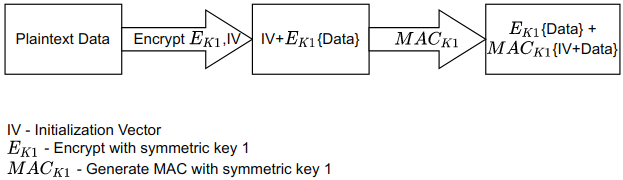
\includegraphics[width=1\textwidth]{./Images/arch-encrypt.png}}
	\subfigure[Decrypt data and verify authentication with K1 key]{\label{fig:arch-decrypt}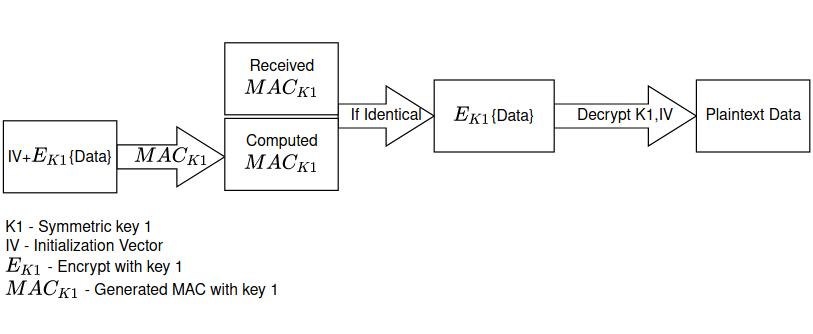
\includegraphics[width=1\textwidth]{./Images/arch-decrypt.png}}
	\caption{Procedure to secure data with authentication and confidentiality}
\end{figure}

Beginning with figure~\ref{fig:arch-encrypt}. The plaintext data sent to the device is first encrypted with the symmetric key \textit{K1}, using a randomly generated \ac{IV}. Then a \ac{MAC} is generated from the encrypted data and \ac{IV}, using the symmetric key. All fragments of information (MAC, IV, ciphertext) are returned to the user, and the user can then send it to other entities in possession of the used \textit{K1} key.

Following with figure~\ref{fig:arch-decrypt}, when a device receives a encrypted message, it computes the MAC of the received \ac{IV} appended with the decrypted data. If the computed and received \ac{MAC} are identical, the ciphertext is decrypted using the same \textit{K1} key and the received \ac{IV}.

Qualified digital signatures provide \textbf{non-repudiation} to a piece of data, using the private key generated inside the box. The user sends the data to the box, and the subsequent signature will be returned as pictured in figures~\ref{fig:arch-ds} and~\ref{fig:arch-ds-verify}.

\begin{figure}[h]
	\centering     %%% not \center
	\subfigure[Alice generates signature of a document]{\label{fig:arch-ds}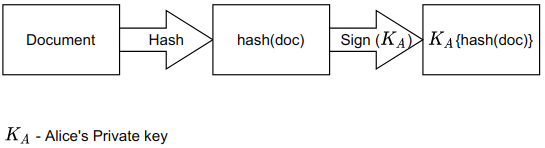
\includegraphics[width=0.7\textwidth]{./Images/arch-ds.png}}
	\subfigure[Bob verifies the signature of the document]{\label{fig:arch-ds-verify}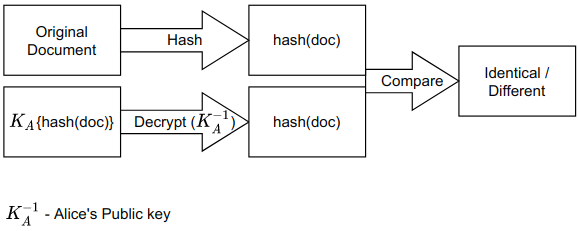
\includegraphics[width=0.7\textwidth]{./Images/arch-ds-verify.png}}
	\caption{Procedure to generate and verify a qualified digital signature}
\end{figure}

The signature is generated by calculating the hash of the data, and signing the digest with the device's private key. To verify a signature (figure~\ref{fig:arch-ds-verify}), the device decrypts the hash with the signer's public key. Next, it computes the hash of the original document, and compares both hashes. If they are identical, the qualified signature is valid.

% -----------------------------------------------------
\subsection{Communication Management}\label{chap:arch:ops:key}

These operations will manage the necessary symmetric keys for secure communications and digital signatures.
% Supported key management operations are: symmetric key generation, symmetric key revocation, if communications are suspected to be compromised, and importation of other entities' keys.
Supported management operations include generation of new symmetric keys for communication and revocation of existing keys saved in the device, if communications are suspected to be compromised.
These operations are only available in the scenario where each device has a pair of asymmetric keys, and there is a protocol in place to distribute public keys.

An entity receives their device, prepared to communicate with other entities, and a list of information of other entities, available to create communications. This information, namely the entities public key, can be imported into the device to generate new keys.
% After the key is imported, a secure connection with a new entity can be established, by sharing symmetric keys.
In order for an entity to communicate with a another entity, with no previously established communications, their device will generate a new symmetric key and store it in secure storage, or in non-volatile memory, encrypted with the device's public key.
Figures~\ref{fig:arch-ecdh-alice} and \ref{fig:arch-ecdh-bob} illustrate the procedure Alice and Bob devices go through to generate new communication keys.

\begin{figure}[h!]
	\centering     %%% not \center
	\subfigure[Alice generates key]{\label{fig:arch-ecdh-alice}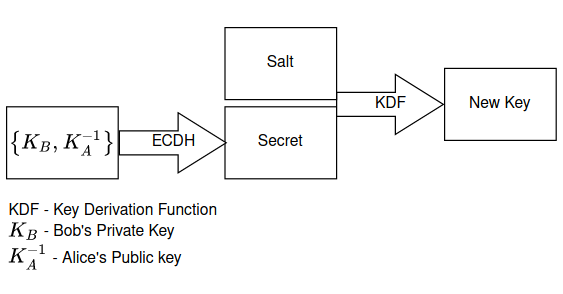
\includegraphics[width=0.65\textwidth]{./Images/arch-ecdh-alice.png}}
	\subfigure[Bob generates the same key]{\label{fig:arch-ecdh-bob}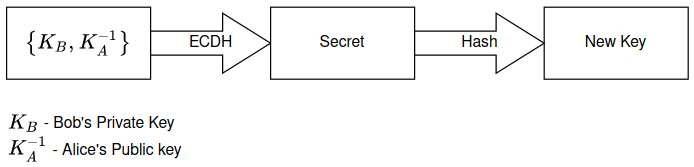
\includegraphics[width=0.65\textwidth]{./Images/arch-ecdh-bob.png}}
	\caption{Alice and Bob generate new key from both asymmetric key pairs}
\end{figure}

The procedure is the same from the perspective of both devices. Alice's device has its private key and the Bob's public key. Bob's device has its private key and Alice's public key. Both generate the same secret from these values using the \ac{ECDH} algorithm, introduced in section \ref{chap:background:crypto:ecdh}.
This secret then serves as input to a key derivation function to derive a new key. This function receives the secret and a public know parameter, a salt, to generate a new key. Alternatively a hashing function such as SHA-256 can be used, but a key derivation function which takes a salt parameter is preferred, so multiple keys can be derived from the same secret.

%The key is first signed with the sender's private key, which is stored in the device's secure storage, and then ciphered with the receiver's public key, which was imported before. Portrayed in figure~\ref{fig:arch-ecdh-bob}, Bob's device decrypts the message using its private key, and decrypts it again with Alice's public key. Finally the key is securely stored in the device, and both entities can subsequently establish secure communications.

When a symmetric key is revocated, due to reaching its expiration date, or from being compromised, entities can generate a new one, using the aforementioned procedure, with an additional parameter for the key derivation function, to generate a completely new and unique key.
